\documentclass[12pt]{ieeeconf}      % Use this line for a4

\include{utilities}
\usepackage{textcomp}
\usepackage{gensymb}
\usepackage{graphicx}
\usepackage{amsmath}
\usepackage{color, soul}
\usepackage{ragged2e}
\usepackage[english]{babel}
\usepackage[version=3]{mhchem}
\usepackage{chemfig}
\usepackage{multirow}
\usepackage{hyperref} % reference url
\usepackage{float}
\usepackage{tikz}
\usepackage{subfigure}
\usepackage{graphicx}
\usepackage{adjustbox} 
\usepackage{amssymb}% http://ctan.org/pkg/amssymb
\usepackage{pifont}% http://ctan.org/pkg/pifont
\newcommand{\cmark}{\ding{51}}%
\newcommand{\xmark}{\ding{55}}%
\linespread{1.2}
                                                          % paper

\IEEEoverridecommandlockouts                              % This command is only
                                                          % needed if you want to
                                                          % use the \thanks command
\overrideIEEEmargins
% See the \addtolength command later in the file to balance the column lengths
% on the last page of the document


\title{\LARGE \bf
IMDb Movie Credits
}


\author{Andrew \textsc{Chan}, Sorrel \textsc{Dando-Wilson}, Johan \textsc{Larsson H\"ork\'en}, Florence \textsc{Routh},\\ Tom \textsc{Sallis}, \\Mathematical \& Data Modelling III\\
\textit{University of Bristol}\\
\today% <-this % stops a space
}


\begin{document}

\pagenumbering{roman}
\pagenumbering{arabic}

\maketitle


\section{Introduction}
\indent The Internet Movie Database, more commonly known as IMDb \cite{imdb}, is an online database storing information regarding films, television shows and video games. Such information consists of a cast and crew for each production, fictional characters, biographies, plot summaries, trivia and reviews. IMDb allows registered users to submit new material and edit existing entries. Despite the data being regulated the system has succumbed to occasional errors and misuse. Hence, the task at hand is to develop a system whereby existing data can be used to flag up a new credit if it does not fit in with said existing data. In this case, the project is limited to investigating if the recurrence of actors starring in the same movies together can be used to establish the authenticity of information supplied about a new credit (i.e., whether a certain actor did indeed feature in a movie based on whether they have previously co-starred with any of the other actors in said movie in a previous existing credit) and flag up if this does not fit with previously known credits. 
\\
\indent The data chosen to be analysed to uncover this relationship is categorised by actors in relation to movies they have featured in. The structure of the data allows us to analyse the problem as a network, where actors are connected by the movies they have co-starred in. There exists multiple approaches to analyse a network to uncover features of the data, including labelling, clustering, shortest path, PageRank, etc. The basic idea of network analysis independent of approach is to uncover features of the data, then to compare different data points to see how much their features differ. Through comparing the features of newly submitted data to the features of existing data related to the submission, it is possible to determine if the submission is probable or not, and flag thereafter.


\subsection{Assumptions}
\indent Inherent to any model, a number of assumptions have been made.
\begin{enumerate}
\item The data itself was downloadable from `Alternative Interfaces' on the IMDb website \cite{interfaces}. As previously mentioned this consists of information for all movies, television shows and video games. For the sake of this project purely movies will be considered.
\item All the data downloaded from the IMDb website was assumed to be correct and could be implemented as training data.
\item Due to the extensive amount of data provided it was decided to focus on a subset of actors.
\end{enumerate}


\section{Data Mining}
\indent The initial format of the data was text files organised by category; for example, actors, actresses, genres, etc., which as previously stated were downloadable from the IMDb website directly. Due to the size and nature of the data, it was necessary to perform data mining so that patterns and knowledge could be extracted for analysis. The data was hence refined using the following constraints.
\\
\indent The file categorised by `actors' was chosen due to the project limitations and a subset of the data was used for analysis. Hence, the data desired needed to consist of the name of an actor and the list of films said actor has featured in. The data given by the IMDb `actors' database followed the following structure.

\begin{table}[H]
\centering
\begin{tabular}{ll}
``xxxxx"        & = a television series \\
``xxxxx" (mini) & = a television mini-series \\
{[}xxxxx{]}    & = character name \\
$<$xx$>$       & = number to indicate billing position in credits \\
(TV)           & = TV movie, or made for cable movie \\
(V)            & = made for video movie (this category does \\
			   & NOT include TV episodes repackaged for \\
               & video, guest appearances in variety/comedy \\
               & specials released on video, or self-help/ \\ 
               & physical fitness videos)
               \label{structure}
\end{tabular}
\end{table}

\indent To analyse this data, it was necessary to convert it into a more manageable format. This was done using a data parser \cite{parser} taking the plain text database as the input, filtering through the data to map each actor to the credits they have featured in and outputting it as a TSV-file (tab separated value). The format of the data after such filtering was as shown below.

\begin{table}[H]
\centering
\begin{tabular}{lll}
 Simon Pegg		& Shaun of the Dead (2004)	& [Shaun]
\end{tabular}
\end{table}

\indent Still following the same conventions as in the original database. Meaning \textit{Simon Pegg} is the actor name, \textit{Shaun of the Dead (2004)} is the name of the movie (and year released) and [\textit{Shaun}] is the character name, each value separated by a tab.
\\
\indent To be able to use only actors and movies, further filtering was required. This meant ``movies" tagged with (TV) and (V) were removed. Additionally, character names and diacritics were removed in order to obtain the most ideal actor-movie format, which could then be stored into a CSV-file (comma separated value).
\\
\indent After parsing the data it was possible to convert the data into a CSV-file so that the number of movies and their corresponding actors could be counted. Each actor and movie was then given a unique ID number to allow for an easier lookup when creating actor-to-actor connections. Due to the project aim and limitations, movies were not important in our flagging. Hence, looking at the actors submitted into a new entry was necessary and to observe the likelihood of two actors working together, therefore an actor-to-actor connection was most suitable.
\\
\indent It was then possible to produce arrays of actor-to-movies and movies-to-actors using their unique ID numbers rather than the whole movie title/actor name. This was achieved by creating an actor-to-movies connection for the movies said actor featured in, and movie-to-actors connection for the actors featured in said movie in the format of arrays. It was then possible to create an actor-to-actors connection of actors who feature in the same movie. On from this, a pairwise comparison was made to the actors to count the number of times they feature in a movie together and thus the weightings were created.
\\
\indent An actor-to-actor pair could then be produced along with their weighting (number of movies said pair have featured in together), this was the penultimate step to creating an adjacency matrix.


\subsection{Adjacency Matrix}
\indent The outputted data from the data mining consisted of purely actors and their corresponding movies, hence it was then possible to create a weighted adjacency matrix to display the relationships between actors and the number of films they have featured in with all other actors, if any.
\\
\indent An adjacency matrix is a symmetrical matrix which can be used to represent a network or graph. The elements in an adjacency matrix represent whether or not a pair of nodes are adjacent to each other within the network, i.e., whether two nodes (actors) are connected by an edge (if two said actors both featured in the same movie together). \cite{wolfram}
\\
\indent The format of the matrix is such that the indices will be actors against actors. The matrix will consist of weightings representing the number of movies actors have featured in together. For example, if an actor has been in no films with another actor, a value of 0 will be assigned, if they have been in one film together assign a value of 1, if they have been in two films together assign a value of 2 and so on. The diagonal of the weighted adjacency matrix should consist of zeros in accordance to what is justified as an adjacency matrix alongside having the total number of movies one actor has featured in will be of no information in terms of the network graph. An example of such matrix is shown below from using a small subset of six actors.    

\begin{center}
$\begin{bmatrix}

    0       & 0 & 1 & 0 & 0 & 0 \\
    0       & 0 & 0 & 0 & 2 & 0 \\
    1       & 0 & 0 & 0 & 0 & 0 \\
    0       & 0 & 0 & 0 & 0 & 0 \\
    0       & 2 & 0 & 0 & 0 & 1 \\
    0       & 0 & 0 & 0 & 1 & 0 
\end{bmatrix}$
\end{center}

\indent The matrix above shows that node 3 and node 1 have featured in one movie together, therefore assigning them a weight of 1. However, using a matrix of this format is not very space efficient due to the large about of zeros that will be entered.
\\
\indent Using the data to form a matrix such as this will allow for an easier manipulation and analysis of the data alongside a clearer visualisation of the relationships between actors. One such visualisation commonly used in this case would be a heat map, whereby the data within the matrix are represented as colours. This can be viewed in Figure \ref{heatmap}, where the colour depicts the intensity or frequency of actors starring in movies together, for example Actor 35 and Actor 39 have featured in ten movies together. 


\section{Network Theory}
\label{network_theory}
\indent To analyse the properties of the data unveiled in the data mining, the project undertook a network analysis. A network analysis is the study of data represented as graphs $G = (V,E)$, where $V$ is a set of items are known as nodes, sometimes referred to as vertices. The set of $V$ have connections $E$ known as edges \cite{network:structure}. An example of such network can be seen in Figure \ref{network:graph}.
\\
\indent Edges between nodes in a network describe some kind of relationship between the nodes. The edges can have different properties, such as weight (cost) or direction. An edge with a weight usually implies that traversal of that edge infers a cost defined by the weight. A graph containing weighted edges is referred to as a weighted graph, whereas an unweighted graph contains only edges without weight. A graph can be directed or undirected, where the edges of a directed graph can only be traversed in a defined direction \cite{network:structure}. These graph properties can be viewed in Figures \ref{weighted}, \ref{directed} and \ref{undirected}.
\\
\indent In the case of movies, a network can be created where each actor or actress is represented by a node in the graph, and each edge between two nodes imply that two actors are connected, i.e., they have featured in a movie together. The graph can be weighted by the number of movies the connected actors have featured in together. For example, if actor \textit{Simon Pegg} and actor \textit{Nick Frost} are connected by an edge with weight 9, this translates to both actors starring in nine movies together. Whilst, if they are not connected by any edge this would mean they have not featured in any movies together, this can be visualised in Figure \ref{network:actors}.



\section{Network Visualisation}
\indent When a network is created it can be visualised as a graph. But to visualise the graph in a 2D or 3D space, each node needs a position relative to one another. There are many different implementations of how to position the nodes, for instance; position the nodes on the border of a circle, with the edges spanning through the circle, shown in Figure \ref{network:circular}. Position the nodes uniformly at random in the unit square, shown in Figure \ref{network:random}. Position the nodes in an aesthetically pleasing way using the Fruchterman-Reingold force-directed algorithm, shown in Figure \ref{network:spring}.
\\
\indent The Fruchterman-Reingold force-directed algorithm is a modified version of the spring-embedder model by Eades \cite{network:eades}. The basic idea of the spring-embedder is to model the layout of a graph by replacing the nodes with steel rings and the edges with springs, thus modelling a mechanical system. The vertices are placed in some initial layout and released so the spring forces on the rings move the system to a minimal energy state. Fruchterman and Reingold expanded the concept using two main principles for graph drawing.
\begin{enumerate}
\item Nodes connected by an edge should be drawn near to each other.
\item Nodes should not be drawn \textit{too} close together.
\end{enumerate}
Then formulating the optimal distance $k$ between nodes as
\begin{equation}
k = C \sqrt{\frac{\text{area}}{\text{number of vertices}}},
\end{equation}
where the constant $C$ is found experimentally. This layout will henceforth be referred to as spring-layout. \cite{network:spring}


\section{Path Planning}
\label{pathPlanning}
\indent One method for analysing the properties of a network is to calculate the shortest path between nodes. Shortest path algorithms can be implemented in various ways with varied results. The basic idea is to calculate the cost of traversing from one node to another, sometimes through potential intermediate nodes in such case calculating the accumulated cost. The costs in the weighted graph introduced in Section \ref{network_theory} is denoted by the weight of each edge. The shortest path from the start node to the goal node is then defined as the path where the accumulated weight along the path is the smallest, as shown in Figure \ref{network:shortest-path}. In the un-weighted graph instance, the shortest path would mean the path between the start and goal node where the number of intermediate nodes is the smallest \cite{network:shortest_path}.
\\
\indent Shortest path algorithms can usually be generalised to also include related problems, such as longest path, the most reliable path, the largest capacity path, and various routing problems \cite{network:shortest_path}. The algorithms usually output a path of edges to traverse between the start and the goal node, or the total cost of traversal from start to goal node. Path results include minimum spanning trees (MST) and shortest path trees (SPT) \cite{network:trees}. There exists multiple modern implementations of shortest path related algorithms, including Breadth First Search (BFS), Depth First Search (DFS), Prim's algorithm, Dijkstra's algorithm, A* search, etc. The one implemented in this project is Dijkstra's algorithm, due to its known efficiency calculating shortest path in a weighted network, further described in \cite{network:dijkstras}.
\\
\indent The problem of deciding whether or not it is likely for an actor to have participated in a specific movie together with another actor can be approached as a path planning problem. Consider having a network containing actors and actresses as described in Section \ref{network_theory}, connected by edges weighted by the number of movies a pair of actors have featured in together. The probability of two actors featuring in a movie together can be seen as the longest path between those actors, since large longest path means the two actors and their colleagues have featured in many movies together, thus increasing the probability. To counteract long path distances and bias through famous actors, the path length can be analysed together with the number of nodes traversed. Paths with fewer intermediate nodes might have a higher likelihood. This process is explained in Figure \ref{pathplan}.
\\
\indent Applying the same concept to determine whether it is likely that an actor has participated in a movie, consider the credit \textit{Shaun of the Dead}, with the subset of actors \textit{Simon Pegg}, \textit{Kate Ashfield}, \textit{Nick Frost} and \textit{Lucy Davies}. Is it likely that the actor \textit{Lois Maxwell} has also featured in said movie? This can be checked by calculating the longest path between \textit{Lois Maxwell} and each of the existing actors featuring in \textit{Shaun of the Dead} using the weighted network of actors and actresses. 
\\
\indent The longest path calculation will give information about path length and number of nodes visited from \textit{Lois} to each of the four existing actors \textit{Simon}, \textit{Kate}, \textit{Nick} and \textit{Lucy}. The path length and amount of visited nodes can be analysed to determine if it is likely that \textit{Lois} has featured in \textit{Shaun of the Dead}. A suggested method is to look at the mean of path length, if the mean is higher then a certain threshold, then it is likely that \textit{Lois} featured in \textit{Shaun of the Dead}, otherwise not. It is also possible to, for instance, look at maximum or minimum values of path length, or to divide path length by the number of nodes visited. 
\\
\indent To determine a threshold, an analysis of the properties in a dataset can be performed by simulating the longest path distances between actors and movies with a known outcome. A suggested approach is to analyse the properties of the shortest path calculations of the following three groups of people:

\begin{itemize}
\item Actors who have featured in more than one movie together with any other actors in the dataset, referred to as a \textit{famous actor}.
\item Actors who have featured in a maximum of one movie together with other actors in the dataset, referred to as an \textit{unknown actor}.
\item An existing actor in a movie who has been removed from the set of actors in said movie and calculating the distance to the rest of the cast, referred to as an \textit{existing actor}.
\end{itemize} 

\indent The outcomes ought to be higher for famous actors than unknown actors, and existing actors should ideally give a realistic indication. The threshold can for instance be set to the mean of the outcomes, but may be further manipulated depending on desired outcome.

\section{Page Ranking}
\indent The PageRank algorithm is a method used by \textit{Google Search} to measure the relevance and importance of a webpage.  The fundamental assumption is that webpages with higher importance are more likely to receive backlinks from other sites.  Large sites such as \textit{BBC News} have new pages being constantly added, each linking back to its parent homepage \cite{princeton}.  The iterative algorithm is relatively simple and works by assigning a weighted numerical value to each element or page, with the goal of calculating its comparative relevance within the set.  Therefore, webpages with higher quality backlinks (such as \textit{BBC News}) will receive a greater PageRank value \cite{checkpagerank}.  Pages with a high PageRank are well connected and hence more easily discovered.
\\
\indent Originally the algorithm was created with the purpose of ranking search engine results, however it can also be applied to nodes in more general graphical problems.  As previously mentioned, a node represents each actor and they are connected by weighted edges depending on the number of films the pair have starred in together.  The PageRank value gives an indication of the relative importance of each actor/graph node based on its connection with other actors/nodes.  The algorithm updates the PageRank score iteratively according to
\begin{equation}
\textbf{r} = \frac{1-P}{n} + P\Big(\textbf{A$^T$}\;\frac{\textbf{r}}{\textbf{d}}+\frac{s}{n}\Big)
\label{pagerank}
\end{equation}
where $\textbf{r}$ is a vector of PageRank scores, $P$ is a scalar damping, \textbf{A$^T$} is the transpose of the adjacency matrix of the graph, $\textbf{d}$ is a vector containing the out-degree of each node in the graph, $n$ is the scalar number of nodes in the graph, and $s$ is the scalar sum of the PageRank scores for pages with no links \cite{pagerank}.  The scalar damping factor is the probability that a random person surfing the web clicks on a link on the current page, rather than continuing on to another random page – this value is usually 0.85.  For an undirected graph with no ingoing or outgoing edges, the vector $\textbf{d}$ is set to a scalar value of 1.
\\
\indent Actors with a higher PageRank value tend to have a greater reputation due to having starred in a large amount of films alongside having worked with actors of a similar status; hence increasing the likelihood of them starring in a new film with another actor.  If a web page has too many external links, its PageRank does not get diluted however its links are worth less; this is referred to as link dilution \cite{linkdilution}.  In the same way, if actors have been in too many movies, then it is more likely that they are extras rather than main roles.  Edges with greater weightings (or links) are far more valuable.  Figures \ref{linkdilution-B} and \ref{linkdilution-S} show a network diagram for two different actors, $A$ and $B$.  Actor $A$ has starred in films with four other actors on more than one occasion (between 2 and 10 films), whereas actor $B$ has starred in films with eight other actors on only one instance.  Despite actor $B$ starring in double the amount of films as actor $A$, these links (with a weighting of 1) are much less valuable than those of actor $A$.  Therefore due to this link dilution process, actor $A$ will receive a much more valuable PageRank than actor $B$.  This concept shows that the PageRank algorithm takes into account both the weighting and the number of actors with films in common.


\section{Results} \label{results}
\indent All results throughout this projects have been implemented using high-level general-purpose programming language \textit{Python}, with appropriate extensions and packages. The open source project can be viewed at \cite{movie-credits}.

\subsection{Network Analysis}
\indent The results of the network analysis in this project were achieved by running a data mining simulation of the first 100,000 lines of data in the `actors' database; due to the limitations of computing power. The data mining returned an adjacency matrix and a tuple of edges, both mapping actors together by how many movies they have featured in together. The adjacency matrix was of the format 10553x10553, and the edges tuple contained 3219 edge pairs linking to 2910 nodes. Using the tuple of edges, this allowed for a graph to be created using the \textit{NetworkX} package in \textit{Python}. The resulting graph can be viewed in Figure \ref{network:100k}.
\\
\indent To determine which new submissions should be flagged, in the case where the new submission is an actor added to a movie, the path planning approach was implemented. To determine a reasonable threshold, sample data was used to collect longest paths and their amount of nodes visited along the path. The sample data was set up for the movie \textit{Murder}, a movie containing many actors from the sample dataset. Using the approach of calculating distances to \textit{famous}, \textit{unknown} and \textit{existing} actors, introduced in Section \ref{pathPlanning}, the following actors were chosen due to their properties and positioning relative to the other actors in the movie.

\begin{itemize}
\item Famous actor: \textit{Spencer Achtymichuk} (Figure \ref{network:famous})
\item Unknown actor: \textit{Hilary Adamson} (Figure \ref{network:unknown})
\item Existing actor: \textit{Steve Adell} (Figure \ref{network:existing})
\end{itemize}

\indent Due to time constraints, simulations were only made for one actor in each of the groups. The shortest path between \textit{Spencer Achtymichuk} and the alphabetically first actor in the movie, \textit{David Ackroyd}, can be viewed in Figure \ref{network:path}, and a zoomed in version in Figure \ref{network:path-zoomed}. No path was found between \textit{Hilary Adamson} and any of the other actors in \textit{Murder}, due to their relationship as seen in Figure \ref{network:unknown}. When removing \textit{Steve} from the cast of \textit{Murder}, he did not have any other connections to any of the actors left, hence no path could be found to any of the actors in \textit{Murder}, the result can be viewed in Figure \ref{network:path-existing}. The results are summarised for \textit{Spencer} in Table \ref{table:spencer}, for \textit{Hilary} in Table \ref{table:hilary} and for \textit{Steve} in Table \ref{table:steve}.
\\
\indent The results show that famous actors have a longest path a little over five and visit around six nodes. Whilst unknown actors and existing actors do not have any paths to the actors in the current dataset. Due to the nature of the data, the threshold is therefore set to
\begin{equation}
\frac{\text{Longest path}}{\text{Nodes visited}} > 1
\end{equation}
for the \textit{maximum} value of the path planning between a new credential and existing crew.
\\
\indent Using this threshold, tests were performed on a test dataset to determine the performance of the algorithm. The movie \textit{Ma 6-T va crack-er (1997)} was chosen for investigation, using the previous definitions, actors were chosen as:

\begin{itemize}
\item Famous actor: \textit{Walter Abel}
\item Unknown actor: \textit{Samuel Abrahamsen}
\item Existing actor: \textit{Lionel}
\end{itemize}

\noindent Running these actors through the flagging algorithm gave following results:

\begin{table}[H]
\centering
\begin{tabular}{lcc}
Ma 6-T va crack-er (1997) & Flagged & Not flagged \\
Walter Abel &  & \xmark \\
Samuel Abrahamsen & \xmark &  \\
Lionel & \xmark & 
\end{tabular}
\caption{Ma 6-T va crack-er (1997)}
\label{table:results}
\end{table}

\noindent These results should be interpreted as it is likely that \textit{Walter} featured in the movie, but not likely that \textit{Samuel} nor \textit{Lionel} featured, and they have hence been flagged for manual checking.


\subsection{PageRank}
\indent The PageRank scores for each actor can be converted back to their assigned unique ID and sorted into descending order.  It is then possible to output the top actors with most relevance or of highest importance. For example,  Table \ref{pageranktable} shows the top rankings for a subset of 9 actors in descending order.  From this subset actor \textit{Hiroshi Abe} (i) scored the highest PageRank.  Despite actor \textit{Jing Abalos} starring in the highest amount of movies (76 credits), \textit{Jing} scored the lowest PageRank of the subset. This shows that the PageRank algorithm takes into account the weighting of each link, as well as the link dilution, rather than just the number of credits the individual has starred in.
\\
\indent This method can be used alongside the current flagging system to produce a more accurate result.  Therefore if a new credit is added with an actor of high PageRank, it is more likely for this addition to be correct.  However, a less relevant actor with a low PageRank has a smaller likelihood of appearing in this new credit, thus this addition would be flagged.


\section{Discussion}
\indent This project has been very data heavy therefore making it difficult to implement algorithms with sufficiently low computational complexity. The initial data mining can be simulated within a matter of minutes, however mapping the data to an adjacency matrix or list of edges required a much higher computational complexity, which rendered the computing time to hours even on datasets as small as 500,000 actors. The dataset used in this instance is therefore bound to actors with last names beginning with the letter `A' and hence leads to a rather strong bias in the data. The connections between actors in a smaller dataset are considerably less than if the full set of actors was able to be used. 
\\
\indent This behaviour can be viewed in Figure \ref{network:100k}, where a large amount of nodes can be seen, but just a few of them are clustered in the middle. Comparing this to the zoomed in version of the shortest path between \textit{Spencer Achtymichuk} and \textit{David Ackroyd} in Figure \ref{network:path}, the network can be analysed in more detail. It can be seen that most nodes are clustered together in groups of less than five nodes. This concludes that when using this subset of actors there are very few of them that have co-starred with any other actors in more than one movie.
\\
\indent Path planning in this sense becomes very difficult, since there is a very high probability that there will be no connection between the actors. The example of \textit{Spencer Achtymichuk} and \textit{David Ackroyd} from Figure \ref{network:path} was specifically chosen since they both are located within the same cluster. However, when selecting a more distant actor, such as \textit{Hilary Adamson} we directly see that there is no path between \textit{Hilary} and \textit{Spencer}. This means that there is a rather high probability that a new credit will be flagged, since only a small subset of famous actors have connections to more than one movie.
\\
\indent Expanding this concept to using the full dataset of actors (from A to Z, spanning the entire alphabet), the principles uncovered in this project are still applicable. However the algorithms would need refactoring to lower the complexity or much more computational power would need to be available. With a larger dataset there is a bigger probability for \textit{medium famous actors} to reach a connection with other \textit{medium famous actors}. Whilst the small subset of data used to get the results in this project does not show the full properties of the data. The thresholds would need to be re-calculated using another dataset and it would be preferable to use a larger training dataset to determine this threshold. Only one training and one test simulation was performed to collect the results presented in Section \ref{results}, due to time limitation. Using a larger dataset of test data and averaging the results would give a more reliable threshold. 
\\
\indent It is still possible to view the results of this project as successful, since it is very unlikely that an actor having featured in only one movie should have featured in another specific movie. As shown by the flagged results in Table \ref{table:results}. To uncover the likelihood of actors that have featured in only one movie, other features could be analysed, such as genre. 


\section{Further Improvements}
\indent One way to improve upon this project would be to combine actresses and actors to form a much larger and information dense dataset. This increased amount of data would increase the number of relationships to be found and hence reduce potential spurious correlations and improve the performance of the model in terms of the accuracy of the flagging system. This could be easily implemented through combining the file categorised by actresses with the file categorised by actors and passing it through the model in the same manner as mentioned in the report, however due to the extensive size of the file and the computational power required this unfortunately was not achieved.  An alternative method to achieve this could be by using a supercomputer to run the data.
\\
\indent As previously mentioned the data was downloadable from a choice of categories, therefore an alternative approach could be taken, for example investigating into the genres of movies and their relationships with certain actors and actresses say. This could potentially be achieved through machine learning techniques whereby actors and actresses could be separated into clusters based on the genre of the films they tend to feature in. Classifying actors and actresses this way could present useful in terms of a flagging system. For example, if it was known a certain actor only featured in horror films and a new credit was released that was classified as a musical and IMDb was updated to say this actor featured in this movie a classifying system based on genres would flag up this submission as it would be highly unlikely. A classification technique such as this could be applied using other categories supplied on IMDb such as Nationality, Age, etc. \\
\indent One of the initial assumptions for this project was to focus on a smaller subset of actors; in the case of the PageRank this subset was actors who have featured in between seventy and eighty credits.  This was done in order to create a subset of `top actors' that were more likely to feature in similar movies.  An alternative method could be to use the PageRank algorithm to create a reduced subset containing the most relevant and important actors.  This could produce a denser and higher weighted adjacency matrix, thus improving the final results of this project.  Furthermore, actors from the same movie may have similar PageRank scores; therefore the PageRank algorithm could also be implemented using these clusters as part of the flagging system.


\section{Conclusion}
\indent To evaluate the likelihood of flagging, it is possible to visualise a dataset of actors and the movies they have featured in as a network. The network can be visualised as a graph, where the actors are represented by nodes and connected by edges weighted by the amount of movies the actors have featured in together.
\\
\indent To determine if a new submission is likely, it is possible to calculate the longest path distance in the network between the new submission and each of the other actors in the movie of the pending credit. If the features of the longest path correspond to a certain threshold, the submission can be seen as likely and hence can be directly entered into the dataset. Otherwise the credential should be flagged for manual confirmation.
\\
\indent From using a small subset of data, results of shortest path analysis show that it is likely that famous actors have featured in a new movie, but credentials of lesser known actors are usually flagged. 
\\
\indent Using only a subset of data does not show all properties of dataset. The first 100,000 lines of data, as used in the results in the project, show that the majority of actors have only featured in one movie, thus resulting in a high flagging probability. This can still be seen as successful results, since it is unlikely that an actor only starring in one movie, together with other actors that also only have starred in one movie, should star in a new credential. 
\\
\indent To conclude, the method of calculating shortest path distances in a weighted network of actors can be used to uncover the likelihood of actors having featured in a movie together. However, a larger dataset is necessary to reveal the full features of the data.


\pagebreak
\onecolumn


\begin{thebibliography}{99}
\raggedright

\bibitem{imdb}
IMDb\\
\url{http://www.imdb.com}
\newline
[Accessed 21/02/2017]

\bibitem{interfaces}
\emph{Alternative Interfaces}, IMDb\\
\url{http://www.imdb.com/interfaces}
\newline
[Accessed 21/02/2017]

\bibitem{parser}
\emph{Parser for the plain text files from IMDB}\\
\url{https://github.com/dedeler/imdb-data-parser}
\newline
[Accessed 08/03/2017]

\bibitem{wolfram}
\emph{Adjacency Matrix -- from Wolfram MathWorld.}\\
\url{http://mathworld.wolfram.com/AdjacencyMatrix.html}
\newline
[Accessed 7/03/2017]


\bibitem{stats}
\emph{Statistical Inference for Networks}, Graduate Lectures, Prof. Gesine Reinert\\
\url{http://www.stats.ox.ac.uk/~reinert/talks/graduatenetworklectures.pdf}
\newline
[Accessed 06/03/2017]

\bibitem{network:structure}
\textit{The structure and function of complex networks}, M. E. J. Newman - University of Michigan
\newline
[Published 04/08/2006]

\bibitem{network:shortest_path}
\textit{Shortest-path algorithms: Taxonomy and annotation}, Narsingh Deo, Chi-yin Pang - Washington State University
\newline
[Published 01/01/1984]

\bibitem{network:trees}
\textit{Introduction to Algorithms}, Thomas H. Cormen, Charles E. Leiserson, Ronald L. Rivest, and Clifford Stein
\newline
[Published 1990]

\bibitem{network:dijkstras}
\emph{Greedy Algorithms -Dijkstra’s shortest path algorithm}, GeeksforGeeks\\
\url{http://www.geeksforgeeks.org/greedy-algorithms-set-6-dijkstras-shortest-path-algorithm/}
\newline
[Accessed 06/03/2017]

\bibitem{network:spring}
\emph{Graph Drawing by Force-directed Placement}, Thomas M. J. Fruchterman and Edward M. Reingold - University of Illinois
\newline
[Published 1991]

\bibitem{network:eades}
\emph{A heuristic for graph drawing} -  Congressus Numerantium, P. Eades
\newline
[Published 1984]

\bibitem{princeton}
\emph{The Google PageRank Algorithm and How It Works}, Ian Rogers\\
\url{http://www.cs.princeton.edu/~chazelle/courses/BIB/pagerank.htm}
\newline
[Accessed 08/03/2017]

\bibitem{checkpagerank}
\emph{PageRank Checker}\\
\url{http://checkpagerank.net}
\newline
[Accessed 08/03/2017]

\bibitem{pagerank}
\emph{Use PageRank Algorithm to Rank Websites}, MathWorks\\
\url{https://uk.mathworks.com/help/matlab/examples/use-page-rank-algorithm-to-rank-websites.html}
\newline
[Accessed 01/03/2017]

\bibitem{linkdilution}
\emph{What is Link Dilution?}, Anant Patel\\
\url{http://www.blurbpoint.com/blog/what-is-link-dilution-devaluation-google-penguin-recovery/}
\newline
[Accessed 08/03/2017]

\bibitem{movie-credits}
\emph{Movie Credits}, Andrew Chan, Sorrel Dando-Wilson, Johan Larsson H\"ork\'en, Florence Routh, Tom Sallis \\
\url{https://github.com/horken7/movie-credits}
\newline
[Accessed 10/03/2017]

\end{thebibliography}
\newpage
\newpage

\onecolumn
\section{Appendix}
\label{appendix}


\subsection{List of Tables}

\begin{table}[H]
\centering
\caption{Shortest path between Spencer Achtymichuk and the cast of the movie Murder}
\label{table:spencer}
\begin{tabular}{lcc}
 & \multicolumn{2}{c}{Spencer Achtymichuk} \\
 & Longest path & Nodes visited \\
adell steve & 5 & 6 \\
ackroyd david(i) & 5 & 6 \\
abbott bruce (i) & 5 & 6 \\
adams dave (i) & 5 & 6 \\
acovone jay & 5 & 6 \\
adair-rios mark & 23 & 6 \\
abbott philip & 5 & 6 \\
adams mason (i) & 5 & 6 \\
adedunyo obaka & 5 & 6 \\
abercrombie ian & 5 & 6 \\
abbott jeff (i) & 4 & 5 \\
abruzzo ray & 5 & 6 \\
adeyemi ayo & 5 & 6 \\
acheson james (ii) & 5 & 6 \\
adams r.j. & 5 & 6 \\
ackerman robert (i) & 5 & 6
\end{tabular}
\end{table}

\begin{table}[H]
\centering
\caption{Shortest path between Hilary Adamson and the cast of the movie Murder}
\label{table:hilary}
\begin{tabular}{lcc}
 & \multicolumn{2}{c}{Hilary Adamson} \\
 & Longest path & Nodes visited \\
adell steve & 0 & 0 \\
ackroyd david(i) & 0 & 0 \\
abbott bruce (i) & 0 & 0 \\
adams dave (i) & 0 & 0 \\
acovone jay & 0 & 0 \\
adair-rios mark & 0 & 0 \\
abbott philip & 0 & 0 \\
adams mason (i) & 0 & 0 \\
adedunyo obaka & 0 & 0 \\
abercrombie ian & 0 & 0 \\
abbott jeff (i) & 0 & 0 \\
abruzzo ray & 0 & 0 \\
adeyemi ayo & 0 & 0 \\
acheson james (ii) & 0 & 0 \\
adams r.j. & 0 & 0 \\
ackerman robert (i) & 0 & 0
\end{tabular}
\end{table}

\begin{table}[H]
\centering
\caption{Shortest path between Steve Adell and the cast of the movie Murder}
\label{table:steve}
\begin{tabular}{lcc}
 & \multicolumn{2}{c}{Steve Adell} \\
 & Longest path & Nodes visited \\
adell steve & - & - \\
ackroyd david(i) & 0 & 0 \\
abbott bruce (i) & 0 & 0 \\
adams dave (i) & 0 & 0 \\
acovone jay & 0 & 0 \\
adair-rios mark & 0 & 0 \\
abbott philip & 0 & 0 \\
adams mason (i) & 0 & 0 \\
adedunyo obaka & 0 & 0 \\
abercrombie ian & 0 & 0 \\
abbott jeff (i) & 0 & 0 \\
abruzzo ray & 0 & 0 \\
adeyemi ayo & 0 & 0 \\
acheson james (ii) & 0 & 0 \\
adams r.j. & 0 & 0 \\
ackerman robert (i) & 0 & 0
\end{tabular}
\end{table}

\begin{table}[H]
\centering
\caption{The PageRank algorithm on a subset of 9 actors sorted in descending order (i.e., starting from actors with the highest PageRank score).}
\label{pageranktable}
\begin{tabular}{cclc}
Index & Actor ID & Actor Name & Movie Credits\\
3 & 1917 & abe hiroshi (i) & 75\\
7 & 9252 & adair robert (i) & 75\\
1 & 910 & abatantuono diego & 70\\
2 & 3668 & abbott john (i) & 75\\
4 & 3216 & abeille jean & 76\\
5 & 8637 & abrham josef & 71\\
6 & 4591 & acosta rodolfo (i) & 73\\
8 & 2150 & adam alfred (i) & 76\\
9 & 7564 & abalos jing & 76\\
\end{tabular}
\end{table}


\subsection{List of Figures}

\usetikzlibrary{shapes.geometric, arrows}
\tikzstyle{startstop} = [rectangle, rounded corners, minimum width=3cm, minimum height=1cm,text centered, draw=black, fill=red!30]
\tikzstyle{io} = [trapezium, trapezium left angle=70, trapezium right angle=110, minimum width=3cm, minimum height=1cm, text centered, draw=black, fill=blue!30]
\tikzstyle{process} = [rectangle, minimum width=3cm, minimum height=1cm, text centered, draw=black, fill=orange!30]
\tikzstyle{decision} = [diamond, minimum width=3cm, minimum height=1cm, t
\tikzstyle{arrow} = [thick,->,>=stealth]
\begin{figure}[H]
\begin{center}
\begin{tikzpicture}[node distance=2cm]
\tikzstyle{arrow} = [thick,->,>=stealth]
\node (start) [startstop] {Start of project};
\node (pro1) [process, below of=start] {Define the problem};
\node (pro2) [process, below of=pro1] {Data cleaning};
\node(pro3) [process, below of=pro2] {Data mining};
\node(pro4) [process, below of=pro3] {Adjacency matrix};
\node(pro5) [process, below of=pro4] {Network analysis};
\node(pro6) [process, right of=pro4, xshift=3cm] {Heatmap visualisation};
\node(pro7) [process, left of=pro4, xshift=-3cm] {Page Rank Algorithm};


%\node(pro9) [process, left of=pro8, xshift=-3cm] {\begin{tabular}{c} Nationwide behaviour \\ (global dynamics) \end{tabular}};
%\node(pro10) [process, right of=pro1, xshift=3cm] {Heatmap visualisation};
%\node(pro11) [process, below of=pro8] {\begin{tabular}{c} Network simulations \\ (local dynamics) \end{tabular}};


\node (stop) [startstop, below of=pro5] {End of project};
\node (FE) [process, below of=stop] {Further extensions};


\draw [arrow] (start) -- (pro1);
\draw [arrow] (pro1) -- (pro2);
\draw [arrow] (pro2) -- (pro3);
\draw [arrow] (pro3) -- (pro4);
\draw [arrow] (pro4) -- (pro5);
\draw [arrow] (pro4) -- (pro6);
\draw [arrow] (pro4) -- (pro7);

\draw [arrow] (pro5) -- (stop);
\draw[arrow, to path={|- (\tikztotarget)}]
  (pro6) edge (stop);
\draw[arrow, to path={|- (\tikztotarget)}]
  (pro7) edge (stop);
\draw [arrow] (stop) -- (FE);

\end{tikzpicture}
\end{center}
\caption{Flow chart to show the steps taken throughout the project.}
\label{flow}
\end{figure}

\begin{figure}[H]
  \begin{center}
   \includegraphics[width=.65\textwidth]{figures/figure_1.png}
    \caption{Heat map to visualise adjacency matrix of seventy `top' actors}
    \label{heatmap}
  \end{center}
\end{figure} 

\begin{figure}[H]
\begin{center}
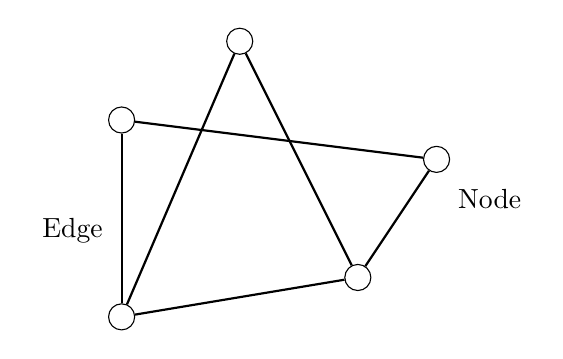
\begin{tikzpicture}
  [every node/.style={circle,fill=white,draw}]
  \node (n4) at (1,6)  {};
  \node (n5) at (1,3.5)  {};
  \node (n1) at (2.5,7) {};
  \node (n2) at (4,4)  {};
  \node (n3) at (5,5.5)  {};
  \node[draw=none,right=.1cm] at (-0.3,4.6) (a) {Edge};
    \node[draw=none,right=.1cm] at (5,5) (a) {Node};

  \foreach \from/\to in {n4,n4/n5,n5/n1,n1/n2,n2/n5,n2/n3,n3/n4}
    \draw[thick] (\from) -- (\to);
\end{tikzpicture}
\caption{A small example network with five nodes, also known as vertices, and six edges.}
 \label{network:graph}
\end{center}
\end{figure}

%%%%%%%

\begin{figure}[H]
\begin{center}
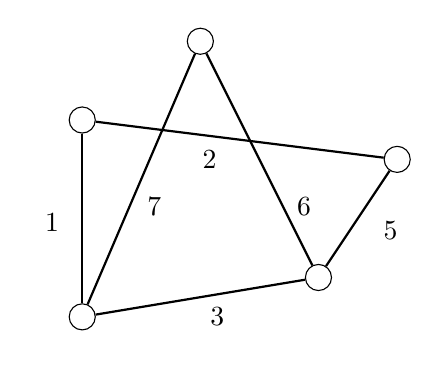
\begin{tikzpicture}
  [every node/.style={circle,fill=white,draw}]
  \node (n4) at (1,6)  {};
  \node (n5) at (1,3.5)  {};
  \node (n1) at (2.5,7) {};
  \node (n2) at (4,4)  {};
  \node (n3) at (5,5.5)  {};
  \node[draw=none,right=.1cm] at (0.2,4.7) (a) {1};
    \node[draw=none,right=.1cm] at (2.2,5.5) (a) {2};
       \node[draw=none,right=.1cm] at (2.3,3.5) (a) {3};
    \node[draw=none,right=.1cm] at (4.5,4.6) (a) {5};
        \node[draw=none,right=.1cm] at (3.4,4.9) (a) {6};
            \node[draw=none,right=.1cm] at (1.5,4.9) (a) {7};

  \foreach \from/\to in {n4,n4/n5,n5/n1,n1/n2,n2/n5,n2/n3,n3/n4}
    \draw[thick] (\from) -- (\to);

\end{tikzpicture}
    \caption{A weighted graph containing nodes connected by weighted edges.}
    \label{weighted}
\end{center}
\end{figure}

\vspace{-3mm}


\usetikzlibrary{shapes.geometric, arrows}
\tikzstyle{arrow} = [thick,->,>=stealth]


\begin{figure}[H]
\begin{center}
\begin{tikzpicture}
  [every node/.style={circle,fill=white,draw}]
  \node (n4) at (1,6)  {};
  \node (n5) at (1,3.5)  {};
  \node (n1) at (2.5,7) {};
  \node (n2) at (4,4)  {};
  \node (n3) at (5,5.5)  {};

  \foreach \from/\to in {n4/n5,n5/n1,n1/n2,n2/n5,n2/n3,n3/n4}
    \draw[thick,arrow] (\from) -- (\to);

\end{tikzpicture}
    \caption{A directed graph containing nodes connected by directed edges.}
    \label{directed}
\end{center}
\end{figure}

\begin{figure}[H]
\begin{center}
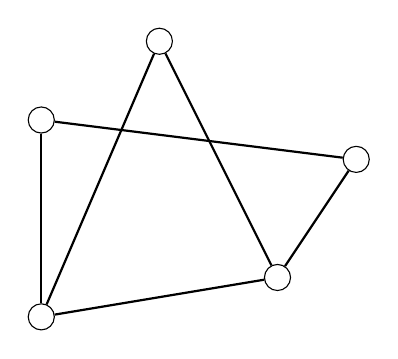
\begin{tikzpicture}
  [every node/.style={circle,fill=white,draw}]
  \node (n4) at (1,6)  {};
  \node (n5) at (1,3.5)  {};
  \node (n1) at (2.5,7) {};
  \node (n2) at (4,4)  {};
  \node (n3) at (5,5.5)  {};


  \foreach \from/\to in {n4,n4/n5,n5/n1,n1/n2,n2/n5,n2/n3,n3/n4}
    \draw[thick] (\from) -- (\to);

\end{tikzpicture}
    \caption{An undirected and unweighted graph containing nodes connected by edges.}
 \label{undirected}
\end{center}
\end{figure}

\begin{figure}[H]
\begin{center}
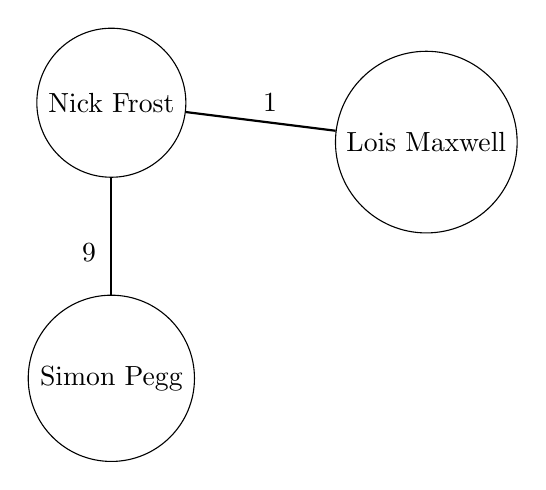
\begin{tikzpicture}
  [every node/.style={circle,fill=white,draw}]
  \node (n4) at (1,6)  {Nick Frost};
  \node (n5) at (1,2.5)  {Simon Pegg};
  \node (n3) at (5,5.5)  {Lois Maxwell};
            \node[draw=none,right=.1cm] at (2.6,6) (a) {1};
            \node[draw=none,right=.1cm] at (0.3,4.1) (a) {9};
  \foreach \from/\to in {n4,n4/n5,n5/n5/n3,n3/n4}
    \draw[thick] (\from) -- (\to);
\end{tikzpicture}
\caption{A small network of actors and actresses, where Nick frost has performed nine movies together with Simon Pegg and one movie together with Lois Maxwell. But Simon Pegg and Lois Maxwell has not performed any movies together.}
 \label{network:actors}
\end{center}
\end{figure}

\begin{figure}[H]
  \begin{center}
   \includegraphics[width=.5\textwidth]{figures/network-circular}
    \caption{The Figure show a network plotted with the nodes (red) positioned on the border of a circle, with edges (black) spanning the circle.}
    \label{network:circular}
  \end{center}
\end{figure} 

\begin{figure}[H]
  \begin{center}
   \includegraphics[width=.5\textwidth]{figures/network-random}
    \caption{The Figure show a network plotted with the nodes (red) positioned randomly inside the unit square, connected by edges (black).}
    \label{network:random}
  \end{center}
\end{figure} 

\begin{figure}[H]
  \begin{center}
   \includegraphics[width=.5\textwidth]{figures/network-spring}
    \caption{The Figure show a network plotted with the nodes (red) positioned in an estetically pleasing way using the Fruchterman-Reingold force-directed algorithm, connected by edges (black).}
    \label{network:spring}
  \end{center}
\end{figure} 

\begin{figure}[H]
  \begin{center}
   \includegraphics[width=.5\textwidth]{figures/ShortestPath2}
    \caption{The Figure show the shortest path between node A and node F.}
    \label{network:shortest-path}
  \end{center}
\end{figure} 


\begin{figure}[H]
\centering
\begin{tikzpicture}
  [every node/.style={circle,fill=white,draw}]
  \node (n4) at (4.5,4)  {D};
  \node (n5) at (1,1.5)  {A};
  \node (n1) at (3,5) {E};
  \node (n2) at (4.5,2)  {B};
  \node (n3) at (3,3)  {C};
    \node (n6) at (1,6)  {G};
        \node (n7) at (4.5,6)  {F};


  \node[draw=none,right=.1cm] at (0.2,4) (a) {5};
    \node[draw=none,right=.1cm] at (2.2,1.2) (a) {1};
      \node[draw=none,right=.1cm] at (3.2,2.3) (a) {1};
            \node[draw=none,right=.1cm] at (3.5,3.2) (a) {1};
                  \node[draw=none,right=.1cm] at (3.2,4.2) (a) {1};
                  \node[draw=none,right=.1cm] at (3.6,5.1) (a) {1};
                        \node[draw=none,right=.1cm] at (2,5.6) (a) {1};


  \foreach \from/\to in {n5/n2,n2/n3,n3/n4,n4/n1,n1/n7,n7/n6,n5/n6}
    \draw[thick,arrow] (\from) -- (\to);

\end{tikzpicture}
\caption{The path from A to G can be seen as either [A,G] = 5 or [A,B,C,D,E,F] = 6. When calculating the path between two actors in a network weighted by how many movies the actors have performed together, it is unclear if it is most likely that the actors have performed a movie together if the path between them is short - or long with higher weight.}
\label{pathplan}
\end{figure}

\begin{figure}[H]
\centering
\begin{tikzpicture}
  [every node/.style={circle,fill=white,draw}]
  \node (n1) at (0,0)  {A};
  \node (n2) at (3,0)  {};
  \node (n3) at (-3,0)  {};
  \node (n4) at (0,3)  {};
  \node (n5) at (0,-3)  {};
            \node[draw=none,right=.1cm] at (1.2,0.2) (a) {3};
            \node[draw=none,right=.1cm] at (-2,0.2) (a) {4};
            \node[draw=none,right=.1cm] at (-0.15,1.6) (a) {10};
            \node[draw=none,right=.1cm] at (-0.15,-1.8) (a) {2};
  \foreach \from/\to in {n1,n1/n2,n1/n3,n1/n4,n1/n5}
    \draw[thick] (\from) -- (\to);
\end{tikzpicture}
\caption{A heavily weighted graph for some actor, A, who has starred in films with other actors more than once.}
\label{linkdilution-B}
\end{figure}

\begin{figure}[H]
\centering
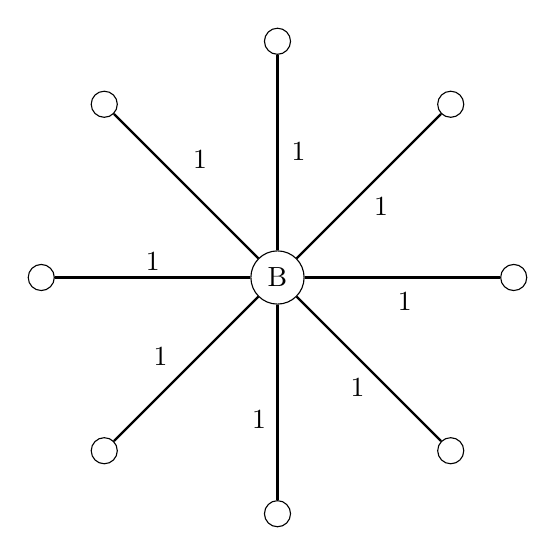
\begin{tikzpicture}
  [every node/.style={circle,fill=white,draw}]
  \node (n1) at (0,0)  {B};
  \node (n2) at (3,0)  {};
  \node (n3) at (-3,0)  {};
  \node (n4) at (0,3)  {};
  \node (n5) at (0,-3)  {};
  \node (n6) at (2.2,2.2) {};
  \node (n7) at (2.2,-2.2) {};
  \node (n8) at (-2.2,2.2) {};
  \node (n9) at (-2.2,-2.2) {};
            \node[draw=none,right=.1cm] at (-0.15,1.6) (a) {1};
            \node[draw=none,right=.1cm] at (0.9,0.9) (a) {1};
            \node[draw=none,right=.1cm] at (1.2,-0.3) (a) {1};
            \node[draw=none,right=.1cm] at (-0.65,-1.8) (a) {1};
            \node[draw=none,right=.1cm] at (-2,0.2) (a) {1};
            \node[draw=none,right=.1cm] at (-1.9,-1) (a) {1};
            \node[draw=none,right=.1cm] at (0.6,-1.4) (a) {1};
            \node[draw=none,right=.1cm] at (-1.4,1.5) (a) {1};
  \foreach \from/\to in {n1,n1/n2,n1/n3,n1/n4,n1/n5,n1/n6,n1/n7,n1/n8,n1/n9}
    \draw[thick] (\from) -- (\to);
\end{tikzpicture}
\caption{An unweighted graph for some actor, B, who has starred in many films with other actors on one occasion.}
\label{linkdilution-S}
\end{figure}

\begin{figure}[H]
  \begin{center}
   \includegraphics[width=.75\textwidth]{figures/network-100k}
    \caption{The Figure show a network of the 100000 first lines of data from the database, plotted in a spring layout.}
    \label{network:100k}
  \end{center}
\end{figure} 

\begin{figure}[H]
  \begin{center}
   \includegraphics[width=.75\textwidth]{figures/network-famous}
    \caption{The actor Spencer Achtymichuk (blue) in relation to the actors in the movie \textit{Murder} (green), in a network of actors.}
    \label{network:famous}
  \end{center}
\end{figure} 

\begin{figure}[H]
  \begin{center}
   \includegraphics[width=.75\textwidth]{figures/network-unknown}
    \caption{The actor Hilary Adamson (blue) in relation to the actors in the movie \textit{Murder} (green), in a network of actors.}
    \label{network:unknown}
  \end{center}
\end{figure}

\begin{figure}[H]
  \begin{center}
   \includegraphics[width=.75\textwidth]{figures/network-existing}
    \caption{The actor Steve Adell (blue) in relation to the actors in the movie \textit{Murder} (green), in a network of actors.}
    \label{network:existing}
  \end{center}
\end{figure}

\begin{figure}[H]
  \begin{center}
   \includegraphics[width=.75\textwidth]{figures/network-path}
    \caption{The shortest path (red) in the network of actors between actor Spencer Achtymichuk (blue) and the alphabetically first actor in the movie \textit{Murder}, David Ackroyd (blue)}
    \label{network:path}
  \end{center}
\end{figure}

\begin{figure}[H]
  \begin{center}
   \includegraphics[width=.75\textwidth]{figures/network-path-zoomed}
    \caption{Zoomed in version on the shortest path (red) in the network of actors between actor Spencer Achtymichuk (blue) and the alphabetically first actor in the movie \textit{Murder}, David Ackroyd (blue)}
    \label{network:path-zoomed}
  \end{center}
\end{figure}

\begin{figure}[H]
  \begin{center}
   \includegraphics[width=.75\textwidth]{figures/network-path-existing}
    \caption{The actor Steve Adell (blue) in relation to the actors in the movie \textit{Murder}, after removing Steve from the cast of the movie.}
    \label{network:path-existing}
  \end{center}
\end{figure}

\end{document}